\documentclass[a4paper,12pt]{article}

\usepackage{graphicx}
\usepackage[utf8]{inputenc}
\usepackage[T1]{fontenc}
\usepackage[francais]{babel}
\usepackage{mathtools}
\usepackage{url}

\author{David Wong
  \and Jacques Monin
  \and Hugo Bonnin}

\title{Whitebox}

\begin{document}

\maketitle

\newpage

\tableofcontents

\newpage


\section{Introduction}

La cryptographie est fondé depuis très longtemps sur le principe que deux personnes veulent converser entre elles sans pouvoir être écouté (Man In The Middle).\\
De nombreux block cipher comme DES ou AES ont étés inventé à travers les années et ont su rester solide contre la cryptanalise. Ces travaux résident sur beaucoup de preuves mathématiques mais aussi sur beaucoup d'observations.

\begin{verbatim}
                         MAN IN THE MIDDLE
                                 |
           .-----.               |               .-------.
           |     |               v               |       |
           | BOB |     ------------------->      | ALICE |
           |     |                               |       |
           .-----.                               .-------.

\end{verbatim}

Avec les avancées technologiques des dernières années de nouvelles utilisation de la Cryptologie ont fait surface. Une assez récente est le besoin d'exécuter du code sur des machines potentiellement dangereuses. Lorsque le code ne contient aucune informations importantes cela n'est pas un problème, mais lorsque le code contient des passwords ou des clefs cela devient un problème.\\

Man at the end : l'attaquant à un accès physique au système. Il peut l'inspecter, lui donner les entrées qu'il veut et analyser les sorties, désassembler le logiciel (IDA), voir les appels au systèmes, voir les accès mémoire, émuler des parties du programme... et finalement en extraire la clef.\\

\subsection{Utilisation}

Avant d'expliquer une potentielle solution à ce problème, voici quelques illustrations afin de mieux comprendre pourquoi on s'intéresse à cette nouvelle utilisation de la cryptologie :



\subsection{Solution}

Whitebox: l'attaquant a encore plus de possibilité puisqu'il contrôle l'environnement: accès à la mémoire, trace, breakpoints,...
Le but est de rendre l'extraction de clef impossible. Pour cela, nous allons prendre un algorithme connu : DES et y appliquer de la tabularisation ainsi que de la délinéarisation qui sont des concepts que nous expliquerons ultérieurement.

\newpage
	
\section{Data Encryption Standard}

Avant de nous lancer dans l'implémentation de la version WhiteBox de DES (Data Encryption Standard), nous avons choisi d'implémenter notre propre version de DES afin de nous familiariser avec son fonctionnement (voir notre algorithme sur GitHub : \url{https://github.com/mimoo/whiteboxDES}).
	
Nous nous intéresserons donc ici au fonctionnement de DES, ainsi qu'à notre approche de son implémentation.

\subsection{Qu'est-ce que DES?}

\subsubsection{Historique et intérêt}

DES est un algorithme de chiffrement symétrique (ou chiffrement par bloc) qui utilise des clés de 56 bits et manipule des blocs de 64 bits. Il a été développé par IBM au début des années 70 à la demande du National Bureau of Standards (NBS) qui proposait de trouver un moyen de sécuriser des informations sensibles, non classifiées, du gouvernement. En 1976, après consultation de la National Security Agency (NSA), Le NBS en sélectionne une version légèrement modifiée, qui sera publiée l'année suivante (le standard arrivant en 1979).

Bien qu'il soit recommandé de ne plus l'utiliser (la dernière version avant l'obsolescence datant de 1999), on peut encore parfois le trouver sous la forme de Triple DES.
	
L'intérêt principal d'utiliser DES dans un contexte de type WhiteBox est que cet algorithme a seulement besoin de transformations linéaires et de substitutions, ce qui facilite l'étude du principe. De plus l'algorithme de Triple DES étant encore parfois utilisé, il peut être intéressant de savoir en implémenter une version WhiteBox.
	
\subsubsection{Génération des 16 clés}	
	
La clé initiale est représentée sur 64 bits (à laquelle on retire 1 bit de parité à chaque octet). 

Un algorithme est utilisé afin de générer les 16 clés (correspondant aux 16 itérations de DES) issues de la clé initiale. 
	
On commence par retirer les 8 bits de parité de la clé (1 bit à chaque octet). La clé obtenue fait alors 56 bits.
\begin{enumerate}
\item Permutation PC1 puis séparation en deux blocs (droite et gauche).
\item Rotation de chaque bloc vers la gauche (le bit en première position passe en dernière position).
\item Fusion des deux blocs
\item Permutation PC2 de 56 bits vers 48 bits qui correspond à la clé du même numéro que l'itération actuelle. On réutilise le bloc de 56 bits (d'avant la permutation PC2) pour la prochaine itération.
\end{enumerate}

Après ces étapes le bloc est chiffré. Pour déchiffrer ce dernier, on utilise le même algorithme, à ceci près que l'on change l'ordre d'utilisation des clés et que l'on inverse les deux blocs de gauche et de droite au début et à la fin de DES.

\begin{figure}[h]
\centering
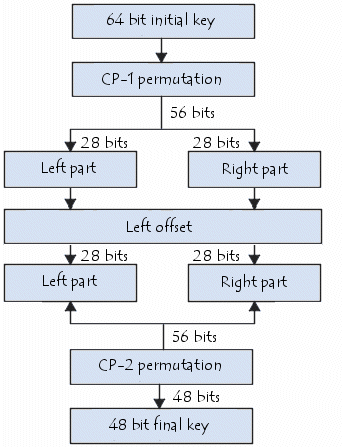
\includegraphics[scale=0.80]{./images/keygen.png}
\caption{Schéma d'une itération de génération de clé}
\label{fig:keygen}
\end{figure}

\clearpage

\subsubsection{Fonctionnement de DES}	

L'algorithme de DES peut se décomposer en 3 grandes étapes :

\begin{enumerate}
\item Une permutation initiale sur le bloc qui est ensuite divisé en deux blocs de 32 bits.

\item S'ensuit un cycle de 16 itérations effectuant les opérations suivantes :
\begin{itemize}
\item Expansion du bloc de droite de 32 bits vers 48 bits (on copie 16 bits du bloc initial, le tout à l'aide d'un table d'expansion). 
\item XOR entre le nouveau bloc de 48 bits et la clé correspondant au numéro d'itération actuelle.
\item Le bloc de 48 bits est divisé en 8 blocs de 6 bits. Chacun de ces sous-blocs passe à travers une table de substitution (qui prend 6 bits en input et donne 4 bits en output). Il y a en tout 8 tables de substitutions, une pour chaque sous-bloc. La valeur en binaire des 4 bits du milieu détermine l'indice de colonne de la table et la valeur binaire des 2 bits extérieurs l'indice de ligne. Le bloc obtenu en fusionnant les 8 sorties de 4 bits a alors une taille de 32 bits.
\item Permutation sur ce bloc (les bits sont changés de place).
\item XOR entre ce bloc et le bloc de gauche.
\item Les deux blocs sont échangés (le bloc de gauche devient celui de droite et inversement).
\end{itemize}


\item Enfin une fusion des deux blocs, suivie d'une permutation finale, inverse de la permutation initiale.
\end{enumerate}

\begin{figure}[h]
\centering
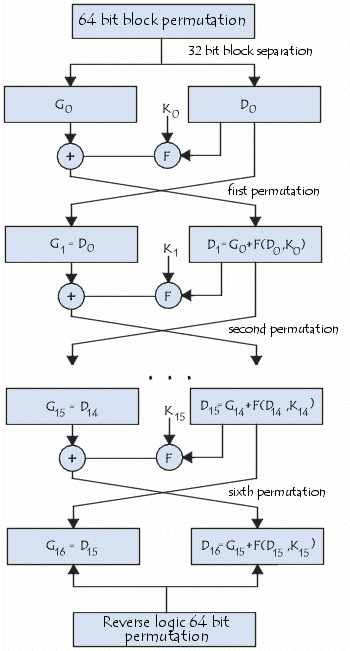
\includegraphics[scale=0.80]{./images/DES_diagram.png}
\caption{Schéma général de DES}
\label{fig:DES-diagram}
\end{figure}

\clearpage

\begin{figure}[h]
\centering
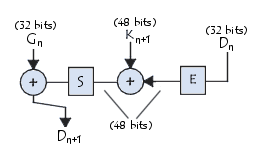
\includegraphics[scale=0.80]{./images/DES_round.png}
\caption{Schéma d'une itération de DES}
\label{fig:DES-round}
\end{figure}

\subsection{Notre implémentation de DES}

vvvvv Toute cette section sujette à modification/suppression vvvvv \\

Dans un soucis de facilité d'utilisation, nous avons créé un générateur de clés de 64 bits. Notre programme comporte donc un fichier genkey (compilé à partir de genkey.c) chargé de générer cette clé. Le programme « desbox » (compilé à partir de DES.h, DES.c et main.c) permet soit d'encrypter (paramètre -e), soit de décrypter (paramètre -d) un fichier passé en entrée. Il prend aussi en argument une clé (paramètre -k) et un fichier de sortie (paramètre -o).

genkey.c :

	Génère une clé aléatoire de 64 bits dont le dernier bit de chaque octet est un bit de parité. S'assure que les clés ne sont pas trop faibles d'un point de vue sécurité en utilisant la fonction key\_schedule() de DES.c (c'est à dire que la période de la clé n'est pas trop faible). Si la clé est trop faible une nouvelle est alors générée et testée à son tour.

DES.c :

	Contient les différentes tables nécessaires au bon fonctionnement de l'algorithme, à savoir les 2 tables de permutation pour la générations des 16 clés, les tables de permutations initiale et finale de DES, ses tables d'expansion, de substitutions et de permutation.
	
	Nous avons choisi de coder nos blocs avec des uint\_64t afin de pouvoir les modifier avec des opérations bit à bit (et donc de gagner en rapidité d'exécution). La fonction addbit() nous sert alors à copier un bit en position x d'un bloc A vers la position y d'un bloc B.
	
	La fonction permutation() peut effectuer (selon le booléen passé en argument) soit la permutation initiale, soit la permutation finale du bloc, en utilisant les tables de permutation correspondantes.
	
	key\_schedule() génère une nouvelle clé à partir de celle passée en argument. Elle demande aussi le numéro d'itération actuel car son comportement diffère entre l'itération numéro 0 et les itérations suivantes. Dans le cas de l'itération numéro 0 on doit commencer par effectuer la permutation PC1. Cette fonction fait appel au tables de permutation PC1 et PC2.
	
	La fonction round() effectue une itération de DES en fonction de la clé passée en paramètre.
	
Elle comprend donc l'expansion, le XOR avec la clé, les substitutions, la permutation et le XOR entre les deux blocs avant de les recombiner. Elle fait appel à la table d'expansion, aux tables de substitutions et à la table de permutation.

main.c :

	Comprend un parseur d'options (clé, encrypter, decrypter, aide, fichier de sortie, fichier d'entrée).


\newpage

\section{Principes et Concepts}

Plusieurs concepts ont étés introduits pour les Whitebox par Chow et cie dans leur article. On peut généralement les diviser en deux parties : l'obfuscation qui cherche à rendre la compréhension du programme plus difficile, et
 l'encryption des entrées/sorties qui cherche à rendre la recherche exhaustive fastidieuse.

\subsection{Partial Evaluation}

On cherche à cacher la clef. La première étape est de pré-calculer toutes les opérations qui sont déjà connu dans notre cas. Puisque dans une whitebox la clef est déjà connu, on pré-calcule toutes les sous-clefs et on cache l'étape du XOR avec ces sous-clefs dans des Lookup tables.

Les lookup tables sont des tableaux qui listent les sorties possibles en fonction des entrées possibles.

\subsection{Tabularizing}

Cette seconde étape consiste à transformer toutes les opérations en Lookup tables.

fonctionnement :

0101 := 5 => L(5) = ?

L = { 0000 => 1, 0001 => 2, ... } comme un tableau

\subsection{Randomization and De-linearization}

aussi appelé I/O-blocked Encoding :

Une fois que toutes les opérations ont étés codés en Lookup tables, il est encore facile de retrouver les matrices qui forment toutes ces transformations et donc d'en extraire la clef. Une façon de rendre ce travail trop fastidieux est d'encoder les entrées et sorties de ces Lookup tables avec des bijections (pour pouvoir les annuler d'une Lookup table à une autre).
Par exemple, si $f_1$ et $f_2$ sont deux lookup tables se suivant ($output = f_2 circ f_1(input)$). On peut rajouter une bijection $E$ entre les deux comme ceci : $f_2 \circ E^-1 \circ E \circ f_1(input)$.

\section{Principes et concepts secondaires}


\subsection{Mixing Bijection}

La création des Lookup tables dans la tabularization se fait à partir de matrices représentant les opérations du cipher. Souvent ces matrices contiennent beaucoup plus de 0 que de 1 ce qui rend les lookup tables trop simples et ce qui crée donc un nouveau problème. Pour éviter ce genre de problème on crée deux opérations au lieu d'une. La première composé d'une bijection. La deuxième composé de son inverse multiplié par l'opération qu'on veut complexifier.\\
Soit $M_1$ la matrice d'une des opérations que l'on transformera en lookup table plus tard. On peut la multiplier par une autre matrice $G$ choisie pertinament pour augmenter le bruit dans $M_1$ (un nombre de 0 et de 1 qui parait aléatoire). De fait que l'opération devienne alors $G \cdot M_1$. Il faut bien sur annuler $G$ ensuite en créant une seconde opération $G^(-1)$.\\
L'opération devient alors : $G^(-1) \cdot (G \cdot M_1)$ où $G \cdot M_1$ est pré-évalué comme une unique opération.

\subsection{By-Pass Encoding}

En général, on veut cacher ce qu'une opération fait. L'idée du bypass est d'élargir la taille de son entré et la taille de sa sortie avec des bits inutiles.

\subsection{Combined Function Encoding}

Lorsque deux opérations sont évalués en même temps, on peut les faire évaluer une entrée composée de leurs deux entrées respectives $(P||Q)(input_P||Input_Q)$.

\subsection{Split-Path Encoding}

lorsqu'on donne un input de n bit, et que l'on reçoit un output de m bits tel que $m < n$ on a une perte d'information. Pour répondre à ce problème on append une fonction prenant le même input pour augmenter le nombre de bit de sorties (faire un schéma ou une formule)

\subsection{External Encoding}

Pour éviter une extraction de l'implémentation de la whitebox, et pour éviter les attaques sur les premiers et derniers rounds, on peut appliquer deux bijections à l'entrée et à la sortie du programme.\\

$E \circ WHITEBOX-DES(input) \circ G$

\section{Implémentation}

Les concepts introduits précédemment sont très théoriques et il faut réfléchir un peu pour les mettre en pratique. Voici notre interprétation:

\subsection{Partial Evaluation}

On crée un programme prenant une clef en entrée et générant toutes les lookup tables dans un fichier qui sera utilisé pour compiler la whitebox plus tard.

\subsection{Tabularizing}

Problème :
On ne peut pas faire des lookup tables trop grosses (3.2) ca augmente exponentiellement.

Pour 8 bits d'entrées il y a $2^{8}$ possibilités. Donc la taille de la lookuptable est de $2^{8}$ octets. ou $2^{8}$ * sizeof(int) puisqu'on utilise int dans notre implémentation.
Pour 16 bits d'entrées, il y a $2^{16}$ possibilités. Donc la taille de la lookup table est de $2^{16}$ octets...

On voit que ca augmente exponentiellement. Il faut donc prendre des lookup tables petites et ne pas faire une énorme lookup table pour notre vecteur de 96 bits.

On crée donc des \textbf{réseaux} de lookup tables.

----

Dans ce même programme on transforme toutes les opérations en \textbf{matrices}.

Chaque matrice est découpé en \textbf{blocs de sous-matrices} et les multiplications des sous-matrices au vecteur associé sont transformées en Lookup tables. On utilise des blocs de matrice assez conséquent pour éviter les blocs nuls (il y a beaucoup de zéros dans ces matrices).

Ensuite tous les XOR sont transformés en Lookup tables aussi qu'on appellera des XOR tables.

Après cette étape toutes les opérations ont étés codés en lookup tables

Par exemple, nous allons décomposer une matrice 16*16 en sous-matrices de 8x4. (selon Link et cie, c'est plus secure).

Voici l'opération sans la décomposition

\begin{figure}[h]
\begin{verbatim}
           .----.     .-------------------.     .----.
           |    |     |                   |     |    |
           |    |     |                   |     |    |
           |    |     |                   |     |    |
           | Y0 |  =  |         M         |  x  | X0 |
           |    |     |                   |     |    |
           |    |     |                   |     |    |
           |    |     |                   |     |    |
           '----'     '-------------------'     '----'

\end{verbatim}
\caption{Avant décomposition en sous-matrice}
\label{fig:ascii-box}
\end{figure}

\clearpage

Voici l'opération après la décomposition en sous-matrice

\begin{figure}[h]
\begin{verbatim}

           .----.     .---------.---------.     .----.
           |    |     |    A    |    B    |     |    |
           | Y0 |     .---------.---------.     | X0 |
           |    |     |    C    |    D    |     |    |
           .----.  =  .---------.---------.  x  .----.
           |    |     |    E    |    F    |     |    |
           | Y1 |     .---------.---------.     | X1 |
           |    |     |    H    |    I    |     |    |
           '----'     '---------'---------'     '----'
           
\end{verbatim}
\caption{Après décomposition en sous-matrice}
\label{fig:ascii-box}
\end{figure}

\clearpage

Chaque sous-matrice va être la source d'une nouvelle lookup table.

Cette lookup table va être créée par le multiplication d'une sous-matrice avec toutes les possibilités d'input.

Elle aura donc $2^8$ = 256 entrées possibles et $2^4$ = 16 sorties possibles.

Ainsi pour une matrice (m,n), et pour une sous-matrice ($m_{1}$,$n_{1}$), il y aura     $\frac{m*n}{m_{1}*n_{1}}$ lookup tables créées qui prendront $(2^{n_{1}})$ valeurs et pourront engendrer $(2^{m_{1}})$ sorties.

\subsection{Randomization}

Pour compliquer la compréhension du programme on peut mélanger l'ordre dans lequel on envois les bits à notre programme. Puisqu'on a les matrices $M_1, M_2 et M_3$, il suffit de les multiplier par d'autres matrices de mélange avant et après.

Par exemple le premier round représenté par notre implémentation :

$M_1 . M_2 . data$

data étant un vecteur de 64bits

peut se remplacer par

$(M_1 . R_1^-1) . (R_1 . M2 ) . data$

* De-linearization :

Une fois que toutes les opérations sont transformés en lookup tables. On rajoute des encodages à ces lookup tables.

Par exemple $L_1$ et $L_2$ deux lookup tables qui se suivent.

$L_1 \circ L_2$

on crée une clef pour $L_1$ et on XOR cette clef à ses sorties. Ce qui fait que $L_1$ ressemble sous le manteau à $output = (L_1(input) \oplus k_1)$

et on décrypte cette encryption dans $L_2$ en faisant un XOR dans ses inputs ($L_2$ ressemble alors à output = $L_2(input \oplus k_1).$

Si $L_1$ sort un octet, et $L_2$ prend un octet en entrée. Alors on a un encodage sur les 256 possibilités de la Lookup table. Ce qui est assez facile à retrouver avec une recherche exhaustive. C'est pourquoi on crée un nombre de Lookup tables différentes pour les XORs assez important pour rendre cette recherche exhaustive inefficace. servir

\newpage

\section{Notre implémentation}

On utilise DES
petite intro

\subsection{Traduction des concepts}

\subsubsection{Bypass}

puisqu'on a, au maximum un état de 96bits dans la mémoire, on va garder cet état de 96 bits tout le long et utiliser les bits qui ne servent à rien comme bypass.

\subsection{Différentes étapes}

\subsubsection{Étape préliminaire}

Avant que les 16 rounds ne s'exécutent, il est nécessaire que les bits d'input subissent une permutation initiale suivie d'une expansion de l'input de 64 bits en 96 bits qui permettra le bypass.
Ces deux opération seront réalisées par une matrice M1 qui ne sera utilisée qu'une fois juste avant les 16 rounds et qui réalisera ceci :

\begin{figure}[h]
\begin{verbatim}

            96b           96x64b           64b
           .----.     .-------------. 
           |    |     |             |     .----.
           |    |     |             |     |    |
           |    |     |             |     |    |
           |    |     |             |     |    |
           | Y0 |  =  |     M1      |  x  | X0 |
           |    |     |             |     |    |
           |    |     |             |     |    |
           |    |     |             |     |    |
           |    |     |             |     '----'
           '----'     '-------------'

\end{verbatim}
\caption{M1 avant décomposition en sous-matrice}
\label{fig:ascii-box}
\end{figure}

\clearpage

Nous décomposons M1 en sous-matrice de taille 4x8. Nous multiplions chacune de ces $\frac{96*64}{4*8}$ = 288 sous-matrices par les $2^8$ = 256 différentes possibilités ayant $2^4$ = 16 résultats possibles.


\subsubsection{Étape 1 à Étape 2}

Nous devons convertir ce fonctionnement :

\begin{figure}[h]
\begin{verbatim}
			
             32b               48b              16b
           ************** ********************* ********
state 1:   *     L(r)   * *       X(r)        * * r(r) *
           ************** ********************* ********
                 |                |      |         |
                 |                v      |         |
                 | *********    .....    |         v
                 | * sK(r) *--> . + .    |    .-------.
                 | *********    .....    '-->(  Merge  )
                 |                |           '-------'
                 |                v               |
                 |         .-------------.        |
                 |          \     S     /         |
                 |           '---------'          |
                 |                |               |
            32b  v                v 32b     32b   v
           ************** *************** ***************
state 2:   *    L(r)    * *    Y(r+1)   * *     R(r)    *
           ************** *************** ***************

\end{verbatim}
\caption{Avant Tabularisation}
\label{fig:ascii-box}
\end{figure}		

\clearpage

En celui-ci :

\begin{figure}[h]
\begin{verbatim}

            *********************************************
state 1:    *          state 1 (12 x 8 = 96 bits)       *
            *********************************************
               |      |      |                       |
               v      v      v                       v
            .-----..-----..-----.                 .-----.
            | T0  || T1  || T2  |       ...       | T11 |
            '-----''-----''-----'                 '-----'
               |      |      |                       |
               v      v      v                       v
            *********************************************
state 2:    *              state 2 (96 bits)            *
            *********************************************			
			
\end{verbatim}
\caption{Après Tabularisation}
\label{fig:ascii-box}
\end{figure}		
		
\clearpage		
		
Pour ce faire, nous allons calculer 12 Lookup Tables qui prendront 8 bits chacun ce qui recouvrira les 96 bits d'input.

Il y a :

8 lookup tables non linéaires qui permettent le xor avec la clef et la substitution en les précalculant.


4 lookup tables linaires qui nous serviront à bypasser les bits qui ne subissent pas de calculs.		
		
\subsubsection{Étape 2 à Étape 3}

\begin{figure}[h]
\begin{verbatim}

           ************** *************** ***************
state 2:   *    L(r)    * *    Y(r+1)   * *     R(r)    *
           ************** *************** ***************
                 |                  |           |
                 v                  |           |
               .....    .--------.  |           |
               . + .<---|    P   |<-'           |
               .....    '--------'              |
                |                               |
            32b '----------------------------------.
                                    |           |  |
                .-------------------|-----------'  |
                |               32b v              v 32b
                |               .-------.       .------.
                |              /  E-box  \     ( Select )
                |  32b        '-----------'     '------'
                |                   |              |
                v               48b v              v 16b
           ************** ********************* ********
state 3:   *   L(r+1)   * *       X(r+1)      * *r(r+1)*
           ************** ********************* ********

\end{verbatim}
\caption{Avant Tabularisation}
\label{fig:ascii-box}
\end{figure}	

\newpage

Comme pour l'étape précédente, nous voulons transformer les différentes opérations de cette étape en look up tables.

Pour ce faire, nous allons modéliser les différentes opérations en matrice puis la décomposer puisque la combinaison de la Permutation et du xor est une fonction affine.

Ces calculs vont être modélisé par M2 qui est une matrice (96,96) et qui réalise :
\begin{enumerate}
\item La permutation
\item Le xor avec la partie gauche
\item L'expansion pour le prochain round,
\item le placement de R(r) dans L(r+1) 
\item l'extraction le vrai R(r).
\end{enumerate}


/!\ A expliquer :

 Y0 = A*X0 [+] B*X1 [+] C*X2 [+] D*X3

\begin{figure}[h]
\begin{verbatim}

     ******  ******    ******  ******
     * X0 *  * X1 *    * X2 *  * X3 *
     ******  ******    ******  ******

        |      |          |       |
        v      v          v       v

        2b    2b          2b     2b
      <----><---->      <----><---->
      .----------.      .----------.
       \   S0   /        \   S1   /
        '------'          '------'
         <---->            <---->
           2b                2b

                \         /
                 \       /
                  |     |
                  v     v

                  2b    2b
                <----><---->
                 .---------.
                 \   S2   /
                  '------'
                   <---->
                     2b

                      |
                      v

                   ******
                   * Y0 *
                   ******

\end{verbatim}
\caption{Avant Tabularisation}
\label{fig:ascii-box}
\end{figure}	
\clearpage

\subsubsection{Étape finale}

L'étape finale va consister à ignorer les bypass (ie, ignorer r(r+1)), inverser la dernière expansion réalisée par M2, échanger L et R en cas de décryptage et faire la permutation finale.

Toutes ces étapes vont être réalisée grâce à une matrice M3 qui va être décomposée en sous-matrice et traduite en Lookup table.
\section{Conclusion}

No secure whitebox implementation known today

\newpage
\section{Bibliographie}


\end{document}
